\section{Software Architecture, Data Model, and What-If Simulation Design}
\label{sec:architecture-data-sim}

\safesubsection{Software Architecture}
\label{subsec:software-architecture}
The Smart E-Mobility Hub is architected as a \textbf{Three-Tier Layered Modular Monolith} (\Cref{fig:architecture}), complemented by a formal UML 2.5 Component Diagram (\Cref{fig:component}) and a Campus Wi-Fi/LAN Deployment Topology (\Cref{fig:deployment}).

\begin{figure}[H]
  \centering
  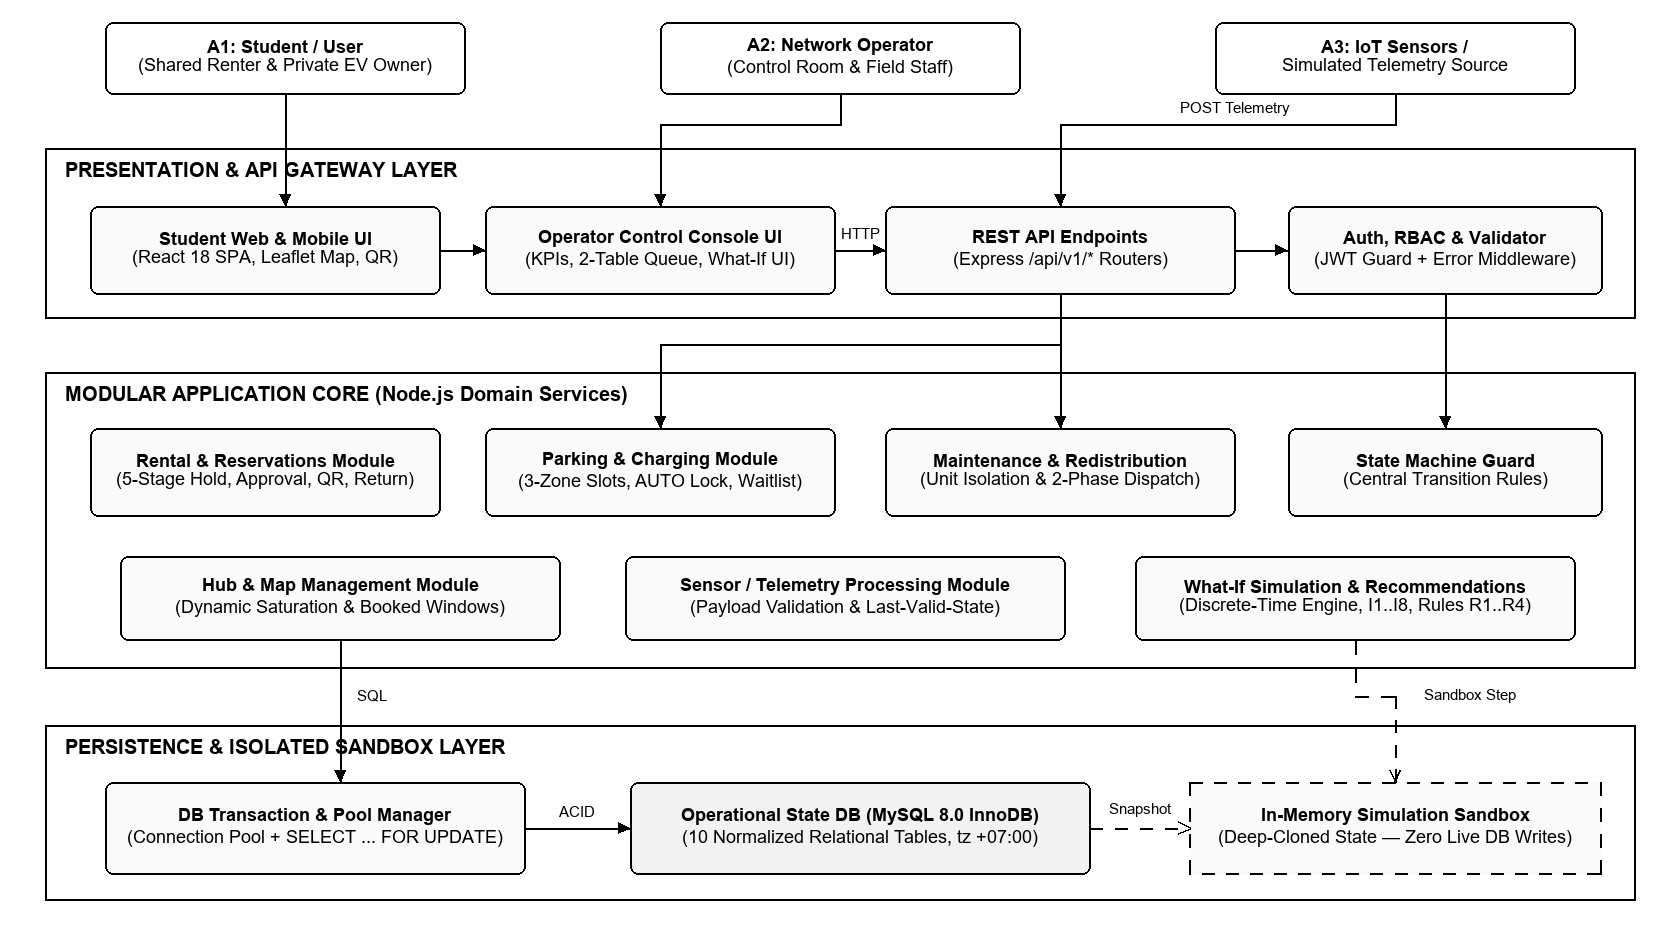
\includegraphics[width=0.95\linewidth]{graphics/diagrams/fig4_1_architecture.png}
  \caption{High-Level Three-Tier Modular Monolithic Software Architecture}
  \label{fig:architecture}
\end{figure}

\begin{itemize}
  \item \textbf{Component Responsibilities:} (1) The \emph{Presentation \& API Gateway Layer} hosts the React 18 Student/Operator SPAs, Express \texttt{/api/v1} REST routers, JWT/RBAC guards, and input/error middlewares; (2) the \emph{Modular Application Core} houses seven cohesive domain modules (\texttt{Rental \& Reservations}, \texttt{Parking \& Charging}, \texttt{Maintenance \& Redistribution}, \texttt{Hub \& Map Management}, \texttt{Telemetry Processing}, \texttt{What-If Simulation}, and the central \texttt{State Machine Guard}); and (3) the \emph{Persistence \& Sandbox Layer} separates transactional MySQL 8.0 InnoDB storage from the ephemeral In-Memory Simulation Sandbox.
  \item \textbf{Communication, Business Logic Location \& Isolation:} External clients communicate via stateless HTTP/JSON REST requests; internal core modules invoke one another synchronously in-process while sharing an InnoDB transaction connection (\texttt{withTransaction}) to enforce multi-table ACID atomicity. \emph{All domain business rules reside strictly inside Application Core services.} What-If runs read a consistent MySQL snapshot and evolve a deep-cloned object graph in RAM (\texttt{0} live DB writes).
\end{itemize}

\begin{figure}[H]
  \centering
  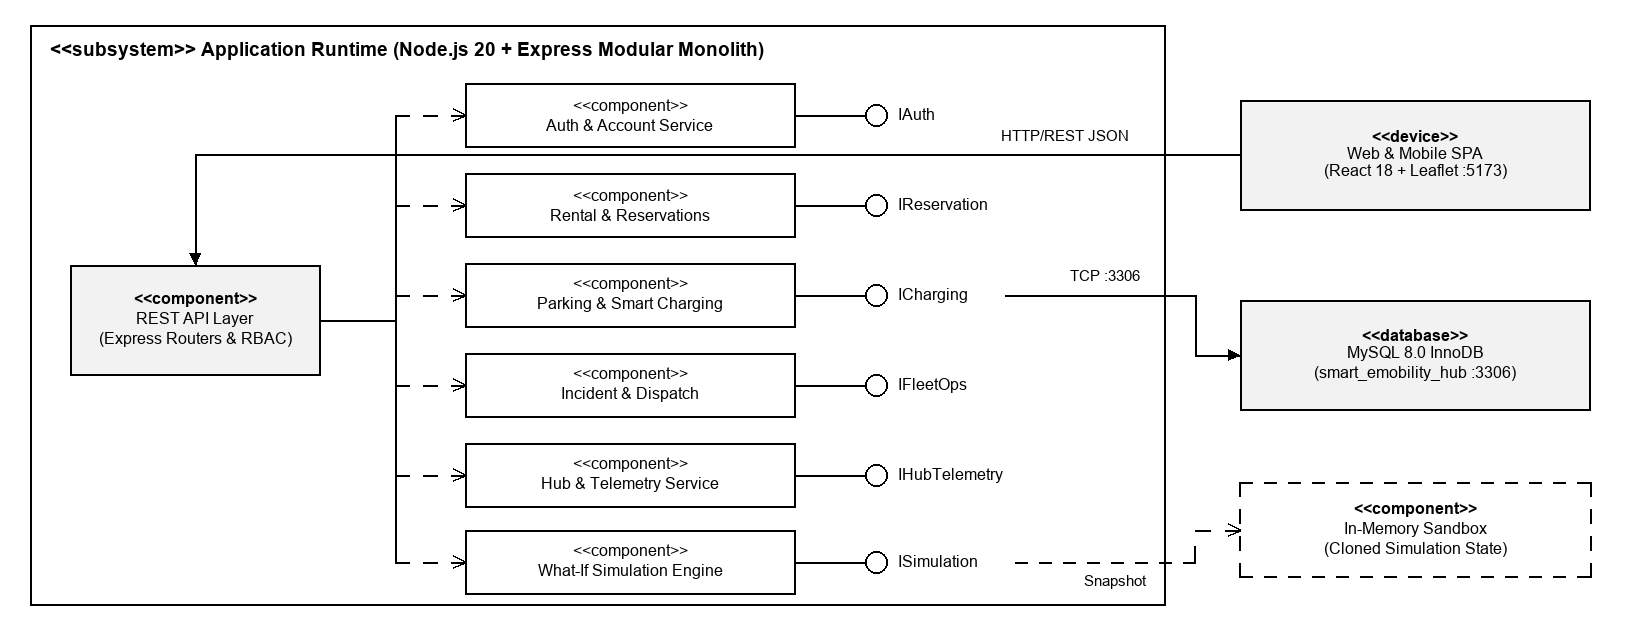
\includegraphics[width=0.92\linewidth]{graphics/diagrams/fig4_2_component.png}
  \caption{UML 2.5 Component Diagram with Provided and Required Interfaces}
  \label{fig:component}
\end{figure}

\begin{figure}[H]
  \centering
  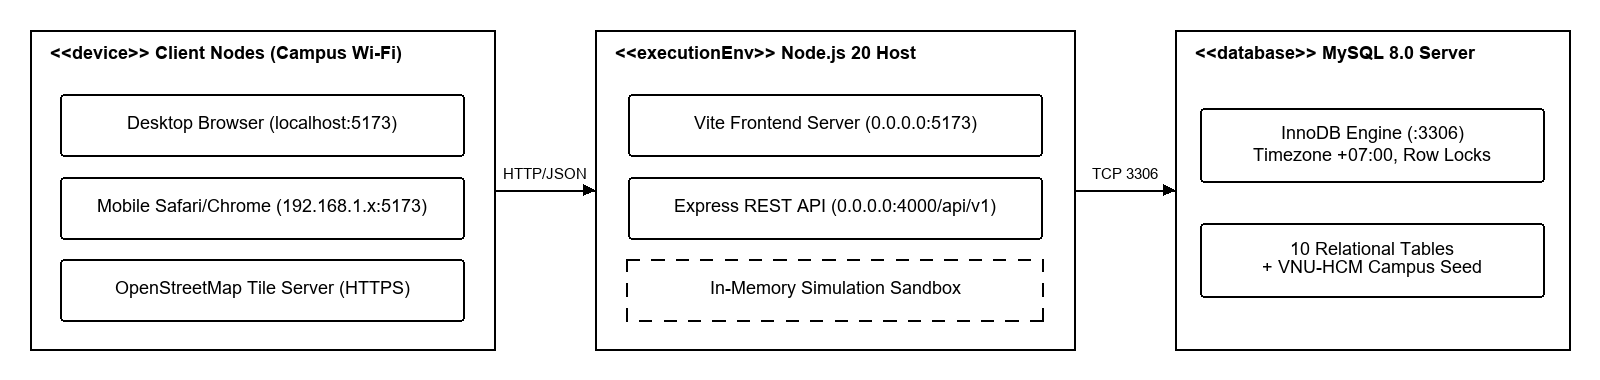
\includegraphics[width=0.92\linewidth]{graphics/diagrams/fig4_3_deployment.png}
  \caption{Campus Wi-Fi / LAN Runtime Deployment Topology}
  \label{fig:deployment}
\end{figure}

\begin{table}[H]
  \centering
  \singlespacing\footnotesize
  \caption{Architectural Comparison and Trade-Off Justification}
  \label{tab:arch-tradeoffs}
  \renewcommand{\arraystretch}{1.23}
  \begin{tabularx}{\textwidth}{|L{3.3cm}|L{4.3cm}|Y|}
    \hline
    \rowcolor{tblHeader}
    \textbf{Architecture Style} & \textbf{Benefits for Project Scope} & \textbf{Trade-Offs \& Selection Decision} \\
    \hline
    \textbf{Three-Tier Modular Monolith + MySQL 8.0 (Selected)} & Single-node InnoDB \texttt{FOR UPDATE} row locks prevent cross-table double-booking; zero inter-service RPC latency; simple campus LAN hosting. & Single-database vertical scaling ceiling and shared Node.js RAM for simulations (mitigated by $30\text{ s}$ cap). \textbf{Selected.} \\
    \hline
    \textbf{Distributed Microservices} & Independent horizontal scaling per domain service. & Requires distributed sagas across Vehicle, Slot, and Hub state updates, creating eventual-consistency race windows. \textbf{Rejected.} \\
    \hline
    \textbf{Document Store (MongoDB)} & Schema-less JSON storage for telemetry logs. & Weaker relational foreign-key guarantees across 10 normalized resource tables. \textbf{Rejected in favor of MySQL 8.0.} \\
    \hline
  \end{tabularx}
\end{table}

\safesubsection{Structural Class Diagram and Physical MySQL 8.0 ERD}
\label{subsec:structural-data}
\Cref{fig:class-diagram} models the implementation-oriented UML Class Diagram (\texttt{<<entity>>}, \texttt{<<service>>}, attributes, operations, and multiplicities), while \Cref{fig:erd} and \Cref{tab:db-tables} specify the 10 normalized MySQL 8.0 InnoDB tables defined in the physical relational schema. Conceptual Phase 2B entities (19 draft classes separating vehicle/parking reservations and simulation logs) were consolidated into 10 normalized tables (\texttt{reservations} unified via \texttt{reservation\_\allowbreak type}; simulation runs held in RAM) to eliminate multi-table join anomalies and enforce strict operational state isolation.

\begin{figure}[H]
  \centering
  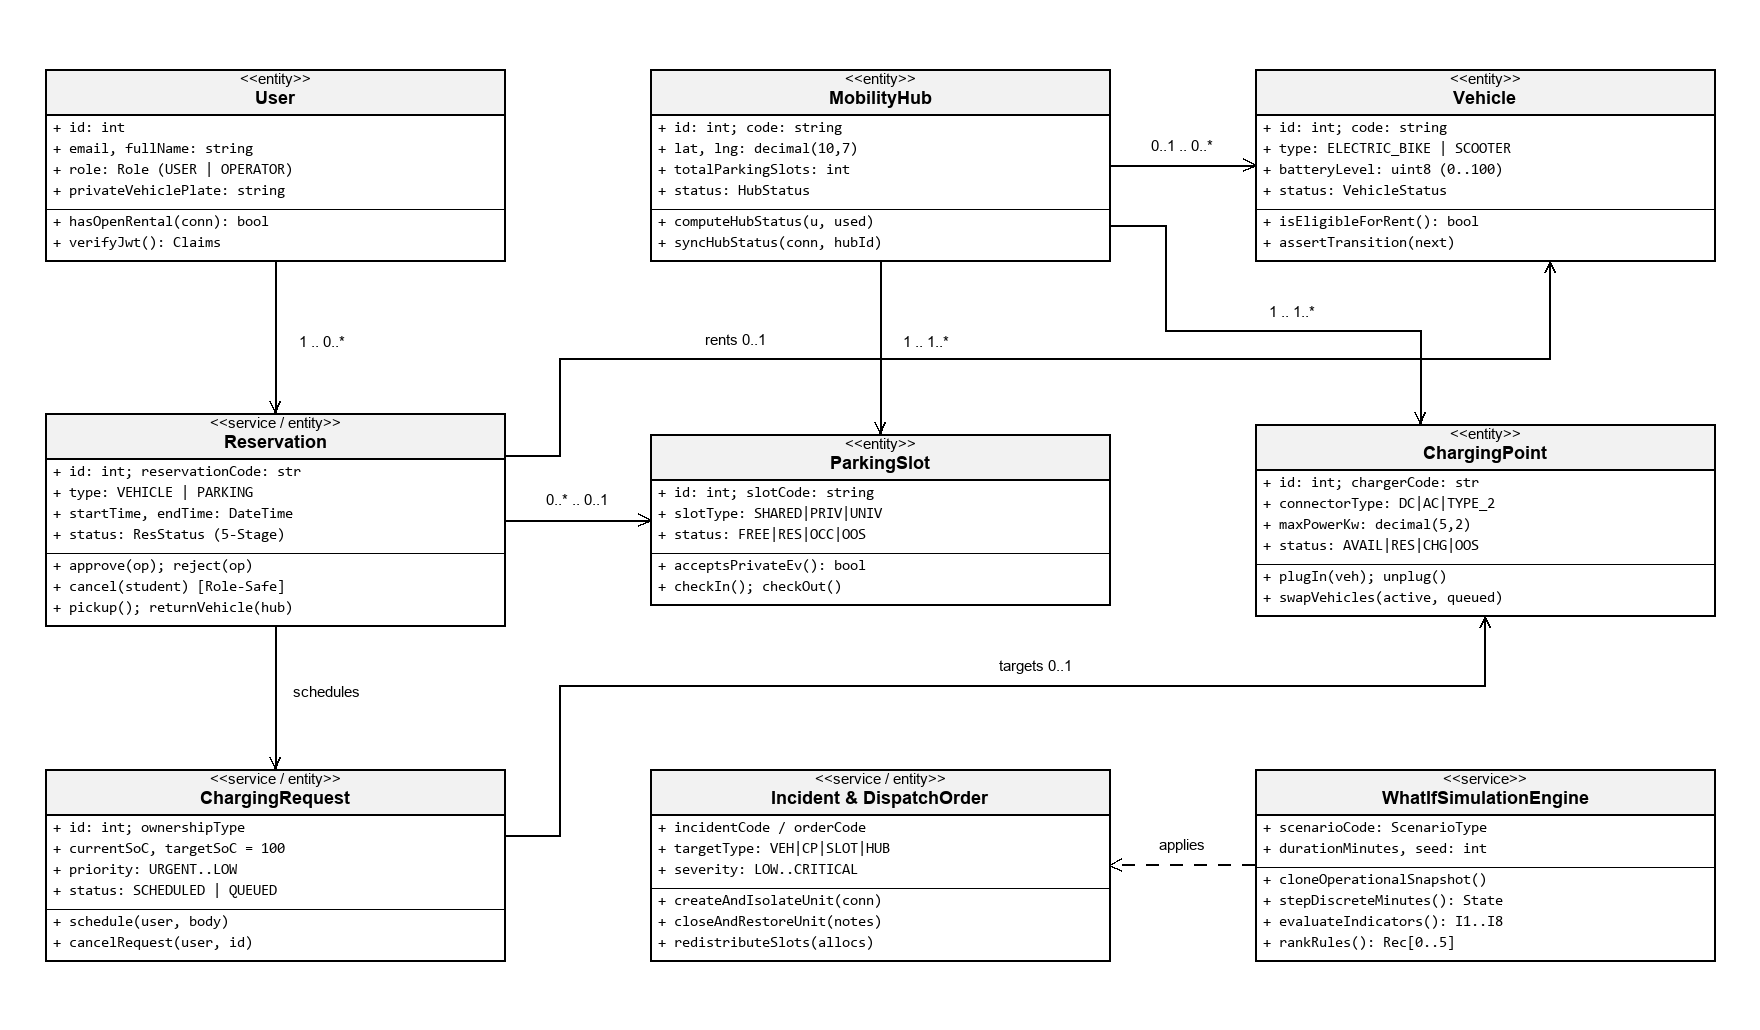
\includegraphics[width=0.92\linewidth]{graphics/diagrams/fig4_4_class_diagram.png}
  \caption{Implementation-Oriented UML Class Diagram}
  \label{fig:class-diagram}
\end{figure}

\begin{figure}[H]
  \centering
  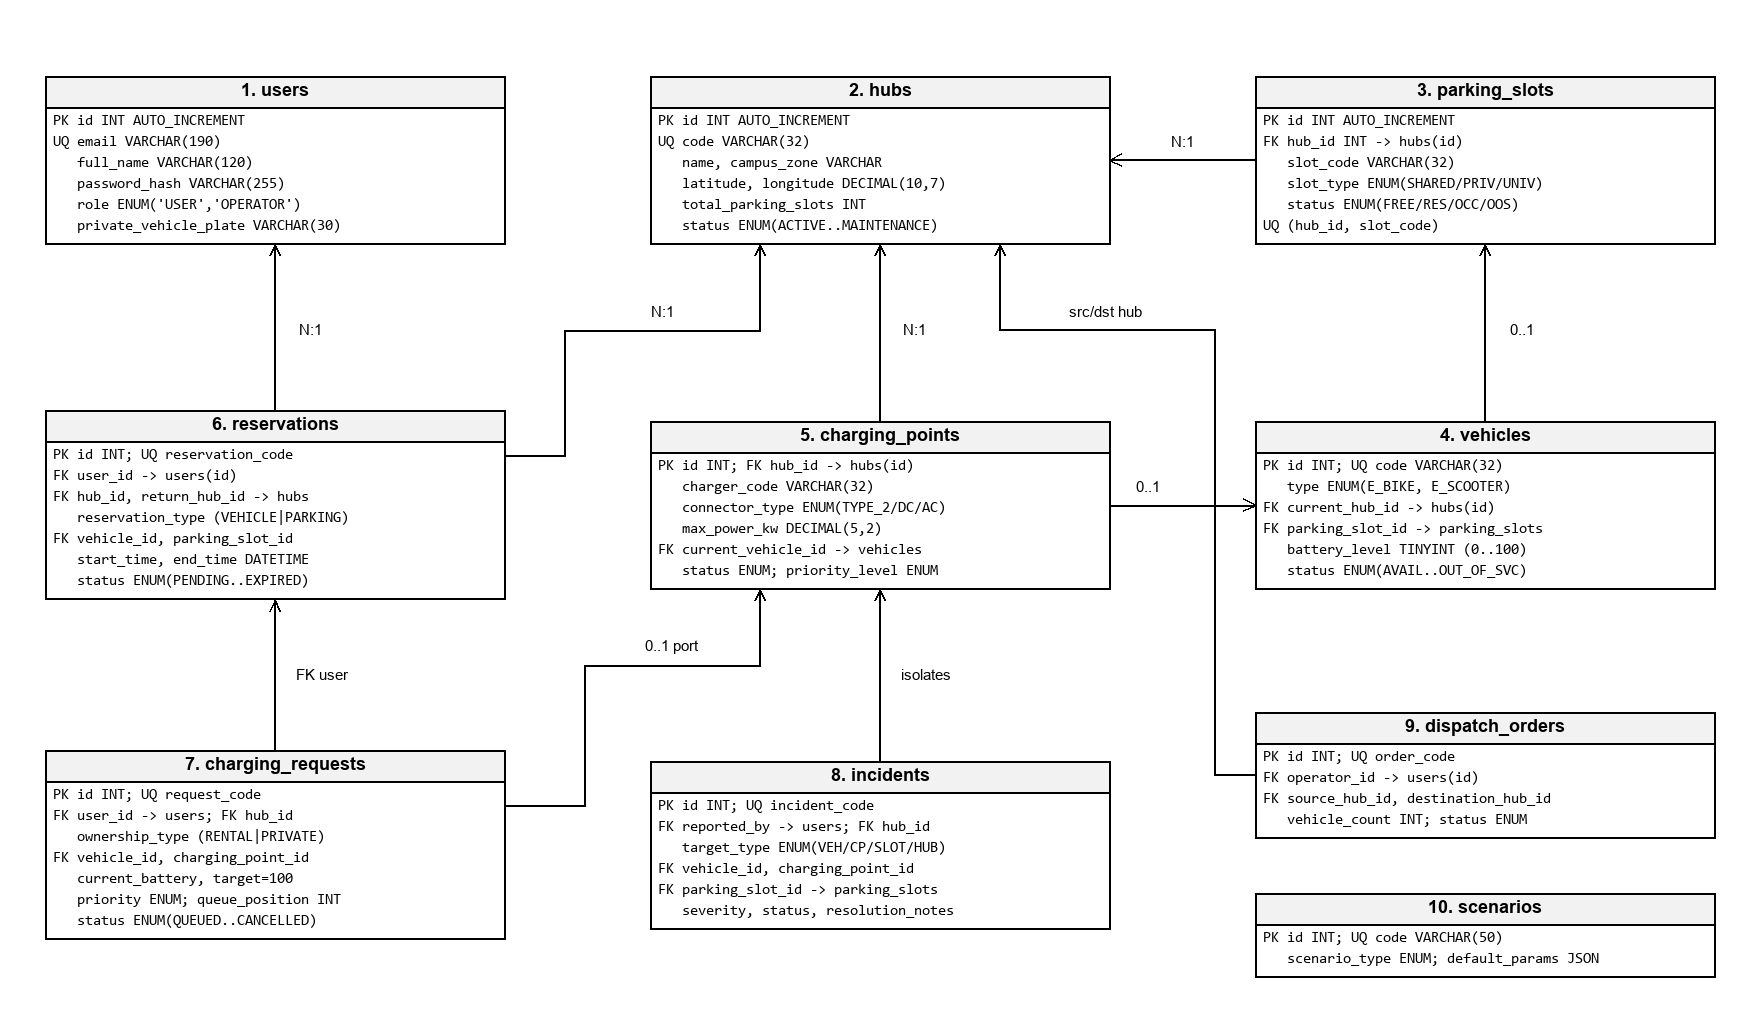
\includegraphics[width=0.92\linewidth]{graphics/diagrams/fig4_5_erd.png}
  \caption{Physical MySQL 8.0 Entity-Relationship Diagram (10 Normalized InnoDB Tables)}
  \label{fig:erd}
\end{figure}

\begin{table}[H]
  \centering
  \singlespacing\footnotesize
  \caption{Physical MySQL 8.0 Relational Tables, Keys, and Domain Roles}
  \label{tab:db-tables}
  \renewcommand{\arraystretch}{1.22}
  \begin{tabularx}{\textwidth}{|L{3.5cm}|L{4.3cm}|Y|}
    \hline
    \rowcolor{tblHeader}
    \textbf{Table Name} & \textbf{Primary \& Key Foreign Keys} & \textbf{Stored Operational State \& Constraints} \\
    \hline
    \texttt{users} & \texttt{PK id}; \texttt{UQ email} & User credentials, RBAC role (\texttt{USER} $|$ \texttt{OPERATOR}), per-user mutex target. \\
    \hline
    \texttt{hubs} & \texttt{PK id}; \texttt{UQ code} & GPS coordinates, capacities, dynamic saturation (\texttt{ACTIVE..MAINTENANCE}). \\
    \hline
    \texttt{parking\_slots} & \texttt{PK id}; \texttt{FK hub\_id};\newline\texttt{UQ(hub, code)} & Zone type (\texttt{SHARED\_\allowbreak EV} $|$ \texttt{PRIVATE\_\allowbreak EV} $|$ \texttt{UNIVERSAL}) and slot state. \\
    \hline
    \texttt{vehicles} & \texttt{PK id}; \texttt{FK current\_\allowbreak hub\_id}, \texttt{slot\_id} & Shared bikes/scooters, $\text{SoC} \in [0,100]$, range, lifecycle status. \\
    \hline
    \texttt{charging\_points} & \texttt{PK id}; \texttt{FK hub\_id},\newline\texttt{current\_\allowbreak vehicle\_id} & Connector type, kW rating, port state (\texttt{AVAILABLE..OUT\_\allowbreak OF\_\allowbreak SERVICE}). \\
    \hline
    \texttt{reservations} & \texttt{PK id}; \texttt{FK user\_id}, \texttt{hub\_id}, \texttt{vehicle\_id}, \texttt{slot\_id} & Unified 5-stage rental \& parking bookings (\texttt{PENDING..COMPLETED/\allowbreak EXPIRED}). \\
    \hline
    \texttt{charging\_requests} & \texttt{PK id}; \texttt{FK user\_id}, \texttt{hub\_id},\newline\texttt{charging\_\allowbreak point\_id} & Scheduled port locks (\texttt{SCHEDULED}) and priority waitlist (\texttt{QUEUED}, $100\%$). \\
    \hline
    \texttt{incidents} & \texttt{PK id}; \texttt{FK reported\_by}, \texttt{hub\_id}, \texttt{unit\_ids} & Mandatory target unit fault logs, severity, status, repair notes. \\
    \hline
    \texttt{dispatch\_orders} & \texttt{PK id}; \texttt{FK operator\_id}, \texttt{src\_hub}, \texttt{dst\_hub} & Audit trail of completed inter-hub and intra-hub EV redistributions. \\
    \hline
    \texttt{scenarios} & \texttt{PK id}; \texttt{UQ code} & Preconfigured JSON parameter templates for What-If simulations. \\
    \hline
  \end{tabularx}
\end{table}

\safesubsection{What-If Simulation and Coordination Design}
\label{subsec:what-if-design}
The What-If subsystem comprises five pipelined modules: \emph{Scenario Validator} $\rightarrow$ \emph{Snapshot Loader} (read-only deep clone of live hubs, EVs, bays, and chargers) $\rightarrow$ \emph{Discrete-Time Engine} ($\Delta t = 1\text{ min}$ seeded step: fault/recovery events, $+1\%/\text{min}$ charging, $-0.4\%/-0.6\%/\text{min}$ trip SoC drain, $20\%$ floor, Poisson demand arrivals) $\rightarrow$ \emph{Impact Evaluator} $\rightarrow$ \emph{Recommendation Engine} (\Cref{tab:sim-scenarios,tab:sim-indicators}).

\begin{table}[H]
  \centering
  \singlespacing\footnotesize
  \caption{Supported What-If Scenarios and Configurable Input Parameters}
  \label{tab:sim-scenarios}
  \renewcommand{\arraystretch}{1.22}
  \begin{tabularx}{\textwidth}{|L{3.9cm}|L{4.2cm}|Y|}
    \hline
    \rowcolor{tblHeader}
    \textbf{Scenario Code / Type} & \textbf{Modeled Operational Stress} & \textbf{Configurable Parameters \& Valid Ranges} \\
    \hline
    \texttt{DEMAND\_SURGE}\newline(\texttt{SCN-METRO-SURGE}) & Peak Metro Line 1 arrival surge of shared-EV requests. & \texttt{targetHubCode}, \texttt{extraDemand\allowbreak Requests} ($5..200$), \texttt{rental\allowbreak Multiplier} ($0.1..5.0$), \texttt{duration\allowbreak Minutes} ($10..1440$). \\
    \hline
    \texttt{HUB\_FULL}\newline(\texttt{SCN-DORMB-FULL}) & Evening return wave saturating Dormitory Zone B parking. & \texttt{targetHubCode}, \texttt{incoming\allowbreak Returns} ($1..100$), \texttt{freeSlots\allowbreak Remaining} ($0..6$), \texttt{inboundBias} ($0.5..5.0$). \\
    \hline
    \texttt{CHARGING\_SURGE} & Simultaneous low-battery recharge spike across hubs. & \texttt{charging\allowbreak Multiplier} ($0.1..5.0$), \texttt{avgInitialSoC} ($15..60\%$), \texttt{timeStep\allowbreak Minutes} ($1..10$). \\
    \hline
    \texttt{CHARGER\_FAILURE}\newline(\texttt{SCN-CHARGER-OUTAGE}) & Partial hardware outage disabling $50\%$ of hub chargers. & \texttt{targetHubCode}, \texttt{failedChargers\allowbreak Count} ($1..N$), \texttt{queuedVehicles} ($0..50$). \\
    \hline
    \texttt{VEHICLE\_IMBALANCE}\newline(\texttt{SCN-FLEET-IMBALANCE}) & $60\%\text{--}80\%$ fleet concentration starving another hub. & \texttt{surplusHubCode}, \texttt{deficitHubCode}, \texttt{imbalance\allowbreak Ratio} ($0.5..0.95$), \texttt{randomSeed}. \\
    \hline
  \end{tabularx}
\end{table}

Overall simulated network stress is ranked using the composite objective function:
\begin{equation}
  \label{eq:sim-score}
  \text{Score} = 0.4 \cdot I_1 + 0.2 \cdot \text{BlockedReturnRate} + 0.2 \cdot \text{NormalizedAvgWait} + 0.2 \cdot I_7
\end{equation}
where lower $\text{Score}$ indicates healthier capacity. Candidate mitigations generated by rules \texttt{R1..R4} (\Cref{tab:sim-indicators}) are simulated against the identical snapshot and seed; actions achieving $\ge 5\%$ $\text{Score}$ reduction are presented as \texttt{Pending} and revalidated against live MySQL constraints if \texttt{A2} confirms execution.

\begin{table}[H]
  \centering
  \singlespacing\footnotesize
  \caption{What-If Impact Indicators (\texttt{I1}--\texttt{I8}) and Coordination Rules (\texttt{R1}--\texttt{R4})}
  \label{tab:sim-indicators}
  \renewcommand{\arraystretch}{1.18}
  \begin{tabularx}{\textwidth}{|C{1.3cm}|L{4.3cm}|Y|}
    \hline
    \rowcolor{tblHeader}
    \textbf{ID} & \textbf{Indicator / Rule Name} & \textbf{Definition or Trigger $\rightarrow$ Recommended Coordination Action} \\
    \hline
    \texttt{I1} & Unmet Demand Rate & Fraction of simulated rental requests rejected due to zero eligible shared EVs. \\
    \hline
    \texttt{I2} & Average Ready Fleet & Mean count of \texttt{AVAILABLE} ($\text{SoC} \ge 20\%$) shared EVs per hub across ticks. \\
    \hline
    \texttt{I3} & Blocked Return Count & Number of inbound vehicle returns rejected because destination bays were full. \\
    \hline
    \texttt{I4} & Peak Hub Occupancy & Maximum parking-slot utilization ratio observed across the simulation window. \\
    \hline
    \texttt{I5} & Mean Charging Queue Delay & Average waiting time (minutes) experienced by \texttt{QUEUED} charging sessions. \\
    \hline
    \texttt{I6} & Charger Port Utilization & Time-averaged fraction of operational charging ports actively delivering energy. \\
    \hline
    \texttt{I7} & Fleet Spatial Imbalance & Dispersion index of available fleet ratios across the four VNU-HCM hubs. \\
    \hline
    \texttt{I8} & Uncharged Backlog Count & Remaining low-battery EVs ($\text{SoC} < 20\%$) still unserved at simulation end. \\
    \hline
    \texttt{R1} & Deficit Fleet Dispatch Rule & Trigger: $I_1 > 0.10$ or stock $< 2$ $\rightarrow$ Transfer \texttt{AVAILABLE} shared EVs from surplus hubs. \\
    \hline
    \texttt{R2} & Smart Priority Promotion & Trigger: $I_5 > 15\text{ min}$ $\rightarrow$ Promote critical/near-ready fleet EVs to \texttt{URGENT} priority. \\
    \hline
    \texttt{R3} & Overflow Evacuation Rule & Trigger: $I_4 \ge 95\%$ or $I_3 > 0$ $\rightarrow$ Relocate idle Zone A EVs to hubs with free bays. \\
    \hline
    \texttt{R4} & Charger Outage Reroute & Trigger: \texttt{CHARGER\_\allowbreak FAILURE} + queue surge $\rightarrow$ Redirect low-SoC EVs to adjacent hubs. \\
    \hline
  \end{tabularx}
\end{table}
